\documentclass[12pt,fleqn]{article}\usepackage{../common}
\begin{document}
Ders 6

Monte Carlo, Entegraller, MCMC

Fizik, biyoloji ve ozellikle makina ogrenimi problemlerinde bazen cok
boyutlu bir fonksiyon uzerinden entegral almak gerekebiliyor. En basit
ornek, mesela bir dagilimin baska bir fonksiyon ile carpiminin beklentisini
(expectation) hesaplamak gerektiginde, ki bu

\[ E(f) = \int p(x)f(x)dx \]

entegralidir, $x \in \mathbb{R}^n$, $p(x)$ dagilim fonksiyonu, $f(x)$ herhangi bir
baska fonksiyon olmak uzere, o zaman tum $x$ degerlerini goz onune alarak
(ayriksal baglamda ya teker teker gecerek, ya da analitik olarak) entegral
hesabini yapmak gerekecekti.

Fakat $p(x)$ bir dagilim olduguna gore, ve bizim gectigimiz her $x$ icin
bir olasilik degeri varsa, bu isi tersine cevirerek, $p(x)$'teki
olasiliklara gore belli (az) sayida $x$ urettirirsek, ve sadece bu $x$'leri
entegral hesabinda kullanirsak yaklasiksal acidan gercek entegral hesabina
yaklasmis oluruz. 

Bu mantikli degil mi? Dusunursek, mesela 10 degeri 0.4 olasiliginda ise, 5
degeri 0.1 olasiliginda ise, hem sayi, hem olasiligi ile carpmak yerine
``daha fazla 10 degeri uretmek'' ve bu degerleri $f$'e gecmek, toplamak,
sonra bolmek, vs. yaklasiksal olarak ayni kapiya cikar. Yani

\[ E_N = \frac{1}{N}\sum_{1=1}^N f(x^{(i)}) \]

ustteki entegralin yaklasiksal temsilidir, $x^{(i)}$ $p(x)$ olasiligina
gore uretilen sayilari temsil ediyor. Ustteki baglantinin teorik olarak
ispati da var, bu ispati burada vermeyecegiz. 

Iste Monte Carlo entegral hesabinin artasinda yatan numara budur. 

MCMC

Demek ki Monte Carlo entegralinin islemesi icin $p(x)$'den ornekleme yapmak
gerekiyor. Simdi ikinci numaraya gelelim. 

Bazen ne yazik ki $p(x)$'den ornekleme yapmak kolay olmuyor. Bu durumlar
icin $p(x)$ yerine onu yaklasiksal olarak temsil eden bir $\pi(x)$'i elde
etmekle ugrasiliyor. Bu $\pi(x)$ ise bir Markov Zincirinin (Markov Chain
-yine MC harfleri!-) duragan dagilimi olarak hayal ediliyor. 

Markov Zinciri teorisinde bir gecis matrisi, yan Markov Zincirinin kendisi
verilir, ve duragan dagilimin hesaplanmasi istenir. MCMC problemlerinde
ise, yani Monte Carlo entegrali icin Markov Zinciri kullanildigi durumlarda
elimizde bir $\pi(x)$ dagilimi vardir ve bir Markov Zinciri olusturmamiz
gerekir. Nihai dagilimi biliriz, ve bu dagilima ``giden'' gecisleri
uretiriz. Bu gecisleri oyle ayarlayabiliriz ki uretilen rasgele sayilar
hedef dagilimindan geliyormus gibi olur. 

Gecisleri uretmek icin literaturde bir cok teknik vardir.  Onemsel
Ornekleme (Importance Sampling), Ornekleme ve Oneme Gore Tekrar Ornekleme
(Sampling Importance Resampling), Metropolis-Hastings, Gibbs Orneklemesi
gibi teknikleri vardir, ve detaylari degisik olsa da hepsi de MCMC
kategorisine girer, ve yapmaya calistiklari $\pi(x)$'e giderken bir sekilde
bir gecisleri, zinciri ortaya cikartmak ve bu gecisleri entegral hesabinda
kullanmaktir.

Ustteki tekniklerden en yaygin kullanilani Metropolis-Hastings
algoritmasidir. 

Sunu vurgulamak onemli, gecisleri uretmek, ``bir tur sanal Markov Matrisi''
yaratmaktir aslinda. Ve her MCMC algoritmasi bunu farkli sekillerde
yapabilir; mesela MH daha basit baska bir dagilim ile ana dagilim arasinda
surekli karsilastirmalar yapar, belli araliklarda gecis yapar, digerlerinde
yapmaz, ve bunun bir yan etkisi olarak ortaya bir Markov Zinciri cikartmis
/ onu kullanmis olur. O gecislerin bir Markov Zinciri'ne esdeger oldugunun
matematiksel olarak ispati da vardir.

Not: Bu alandaki makalelerde bir dagilimin ``belli bir carpimsal sabite
kadar'' bilindigi (known up to a multiplicative constant) soylenir. Bu soz
aslinda su anlama gelir. Mesela ayriksal bir dagilimimiz var, ama bu
dagilimin kendisini, su halini biliyoruz

\verb![ 4.3  2.   8.4  8.7  1.8]!

Bu bir dagilim degil, cunku ogelerin toplami 1 degil. Onu bir dagilim
haline cevirmek icin, tum ogeleri toplamak ve bu vektordeki tum sayilari bu
toplam ile bolmek gerekir. Toplam 25.2, bolersek

\verb![ 0.17063492  0.07936508  0.33333333  0.3452381   0.07142857]!

Ilk vektor ``belli bir carpimsal sabite kadar'' bilinen dagilim, carpimsal
sabit 25.2. Esas dagilim ikinci vektor. 

Peki niye bu sozu soyleyenler toplami hesaplayip gercek dagilimi
hesaplamiyorlar? Sebep performans. Bazen ayriksal dagilim o kadar yuksek
boyutlu, fazla oge iceren bir halde oluyor ki, performans acisindan bu
basit toplam hesabini yapmak bile cok pahali oluyor. Iste MCMC metotlarinin
bir guzel tarafi daha burada, dagilimin kendisi olmasa bile belli bir
carpimsal sabite kadar bilinen versiyonlari ile gayet rahat bir sekilde
isliyorlar.

Metropolis-Hastings

\begin{minted}[fontsize=\footnotesize]{python}
def p(x):
    mu1 = 3; mu2 = 10
    v1 = 10; v2 = 3
    return 0.3*np.exp(-(x-mu1)**2/v1) + 0.7* np.exp(-(x-mu2)**2/v2)

def q(x):
    mu = 5; sigma = 10
    return np.exp(-(x-mu)**2/(sigma**2))

stepsize = 0.5
x = np.arange(-10,20,stepsize)
px = np.zeros(x.shape)
for i in range(len(x)): px[i] = p(x[i])
N = 5000

# independence chain
u = np.random.rand(N)
mu = 5
sigma = 10
y = np.zeros(N)
y[0] = np.random.normal(mu,sigma)
for i in range(N-1):
    ynew = np.random.normal(mu,sigma)
    alpha = min(1,p(ynew)*q(y[i])/(p(y[i])*q(ynew)))
    if u[i] < alpha:
        y[i+1] = ynew
    else:
        y[i+1] = y[i]

# random walk chain
u2 = np.random.rand(N)
sigma = 10
y2 = np.zeros(N)
y2[0] = np.random.normal(0,sigma)
for i in range(N-1):
    y2new = y2[i] + np.random.normal(0,sigma)
    alpha = min(1,p(y2new)/p(y2[i]))
    if u2[i] < alpha:
        y2[i+1] = y2new
    else:
        y2[i+1] = y2[i]

plt.figure(1)
nbins = 30
plt.hist(y, bins = x)
plt.plot(x, px*N/np.sum(px), color='r', linewidth=2)

plt.savefig('stat_mcmc_01.png')
\end{minted}

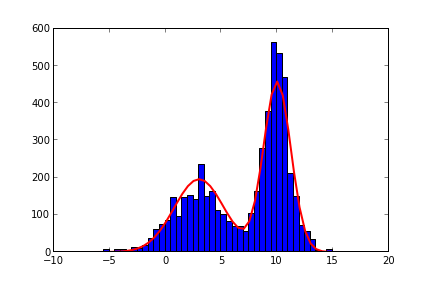
\includegraphics[height=6cm]{stat_mcmc_01.png}

Gibbs Orneklemesi

Bu ornekleme metodu Metropolis yonteminin bir versiyonu olarak kabul
edilir, Metropolis yontemlerinde bir teklif (proposal) dagilimi $Q$ vardir,
ve bu dagilimin orneklenmek istenen $P$ ile iliskisine gore zar atilip elde
edilen yeni nokta kabul edilir, ya da kenara atilir. Gibbs ile de bir $Q$
vardir, ama bir cinlik yapilmistir, $Q$ icin $P$'nin kendisi, daha dogrusu
onun kosullu dagilim hali kullanilir. Bu kosullu dagilim her $i$ icin
$P(x_i|\{x_j\}_{j \ne i}$, burada $x_i$ cok boyutlu $x$'in bir ogesidir,
$\{x_j\}_{j \ne i}$ ise $i$ olmayan diger tum ogelerdir. Yani $i$ {\em
  olmayan} her degisken kosulunda $i$ orneklenir. Bu kullanimin Metropolis
yontemi ile ayni oldugu ispatlanmistir. Kosullu dagilimin kullanilmasinin
ana sebebi ise cok boyutlu $P$ zor bir dagilim olsa bile cogunlukla onun
kosullu ve tek boyutlu dagiliminin rahatca orneklenebilir halde olmasidir.

Algoritma soyle; Rasgele bir baslangic noktasindan baslanir, ve biri harici
tum degiskenler sabit tutulup sabit olmayan degisken orneklenir. Bu islem
surekli uygulanir, bu yapilinca sanki orneklenen dagilimin en olasi yerleri
gezilmis olur. 

Mesela 2 boyutta, bir $x^{(t)}$ noktasindan basladigimizi farzedelim,
$P(x_1|x_2)$ dagilimindan bir $x_1$ orneklenir, $b$ seklinde kosullu
dagilimin tek boyutlu bir Gaussian oldugunu goruyoruz (ki ana dagilim iki
boyutlu Gaussian), bu tek boyutlu dagilimdan bir orneklem aliniyor, dogal
olarak o tek boyutlu dagilimin tepe noktasinin altinda bir yerden.


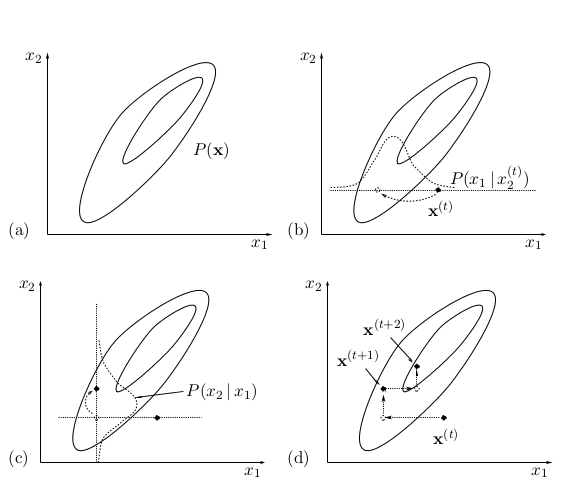
\includegraphics[height=8cm]{gibbs.png}

Sonra bu nokta sabitleniyor (yani yeni bir kosullu dagilim yaratiliyor, ve
orneklenen $x_1$ simdi sag tarafta), yani $P(x_2|x_1)$ dagilimindan. Bu
bizi $x^{(t+1)}$ konumuna (state) goturuyor, bu boyle devam ediyor. $K$
degisken (boyutundaki) iceren bir sistemde, genel formuller soyle,

$$ x_1^{(t+1)} \sim P(x_1 | x_2^{t},x_3^{t},..,x_K^{t}, $$ 

$$ x_2^{(t+1)} \sim P(x_2 | x_1^{t},x_3^{t},..,x_K^{t}, $$ 

$$ x_3^{(t+1)} \sim P(x_3 | x_1^{t},x_2^{t},..,x_K^{t}, $$ 

vs..



Kaynaklar

[1] Algorithmic Machine Learning, Stephen Marsland

[2] Information Theory, Inference and Learning Algorithms, D. MacKay

\end{document}
